%-----------------------------------------------------------------------------
%
%               Template for sigplanconf LaTeX Class
%
% Name:         sigplanconf-template.tex
%
% Purpose:      A template for sigplanconf.cls, which is a LaTeX 2e class
%               file for SIGPLAN conference proceedings.
%
% Guide:        Refer to "Author's Guide to the ACM SIGPLAN Class,"
%               sigplanconf-guide.pdf
%
% Author:       Paul C. Anagnostopoulos
%               Windfall Software
%               978 371-2316
%               paul@windfall.com
%
% Created:      15 February 2005
%
%-----------------------------------------------------------------------------

% Two column, single spaced.
\documentclass[10pt, nocopyrightspace, numbers]{assets/sigplanconf}

% One column, single spaced.
% \documentclass[journal,11pt,onecolumn]{assets/IEEEtran}
% One column, double spaced.
% \documentclass[journal,11pt,onecolumn,draftclsnofoot]{assets/IEEEtran}

% The following \documentclass options may be useful:

% preprint      Remove this option only once the paper is in final form.
% 10pt          To set in 10-point type instead of 9-point.
% 11pt          To set in 11-point type instead of 9-point.
% numbers       To obtain numeric citation style instead of author/year.

\usepackage{nimopaper}

\begin{document}
\title{\textsc{Animate++}: an vector animation library in C++}

% IEEE style author format

% \author{
% \IEEEauthorblockN{Wode ``Nimo'' Ni}
% \IEEEauthorblockA{Columbia University\\
% wn2155@columbia.edu} }  %<------ Line breaks in the current column

% Sigconf author format
\authorinfo{Wode ``Nimo'' Ni}
           {Columbia University}
           {wn2155@columbia.edu}
\authorinfo{Xuanyuan Zhang}
           {Columbia University}
           {xz2580@columbia.edu}
\maketitle


% \begin{abstract}
%     Enter abstract here
% \end{abstract}

% KEYWORDS: Sigconf specific
% \keywords
% Domain-Specific Languages, Language extensibility, Language composability

%------------------------------------------------------------------------------
% Content

\section{Motivation}

Vector graphics with animation has been popular ever since the era of Adobe Flash in the last 2 decades. Recently, an alternative to create vector-based animation,  Structured Vector Graphics (SVG) and HTML5 Canvas has became more popular among front-end developers and artists. The problem with these data formats, however, are often difficult for human to parse and interact with. Therefore, many libraries in JavaScript\cite{paperjs, snapsvg} and direct manipulation tools\cite{svgator} emerged. Sadly, due to JavaScript’s weaker support for object-oriented programming (OOP), the library are sometimes less intuitive to interact with and lack language affordances such as type-checking. The direct manipulation tools, on the other hand, have more user-friendly interfaces but lack high-level abstractions and ways to encode complex behaviors, which can be tedious to work with.

\section{Objective}

The goal of this project is to programmatically create vector animation in an intuitive, object-oriented manner. Taking advantages of C++’s object oriented programming features as well as static typing, we believe our library will bring up an intuitive environment where users compose new vector graphics primitives, import existing ones, and eventually generate beautiful animations in a light-weight manner.

\section{Related Work}

\begin{itemize}
    \item
    \textbf{Snap SVG}: a JavaScript Library with support for creating SVG based animations
    \item
    \textbf{Paper.js}: “The Swiss Army Knife of Vector Graphics Scripting”, another JS library for vector graphics animation. It shows some interesting uses of the JS language: it implemented (a very limited version of) operator overloading in the library, which turns out to be extremely complicated to implement given the JS language. We believe Animate++ can replicate and enhance its effort in simplifying the library interface using C++, which has strong language features.
    \item
    \textbf{SVGator}: a direct manipulation tool to animate SVG files. We plan to learn from it’s user interface and provided functionalities to build our abstractions and library functions to model them. We believe that a programmatic tool will be more powerful in that users can compose customized functions to automate the design process and encode complex behaviors (e.g. complex paths that objects travel) programmatically.
\end{itemize}

\section{Proposed Solution}

\begin{figure}[H]
    \centering
    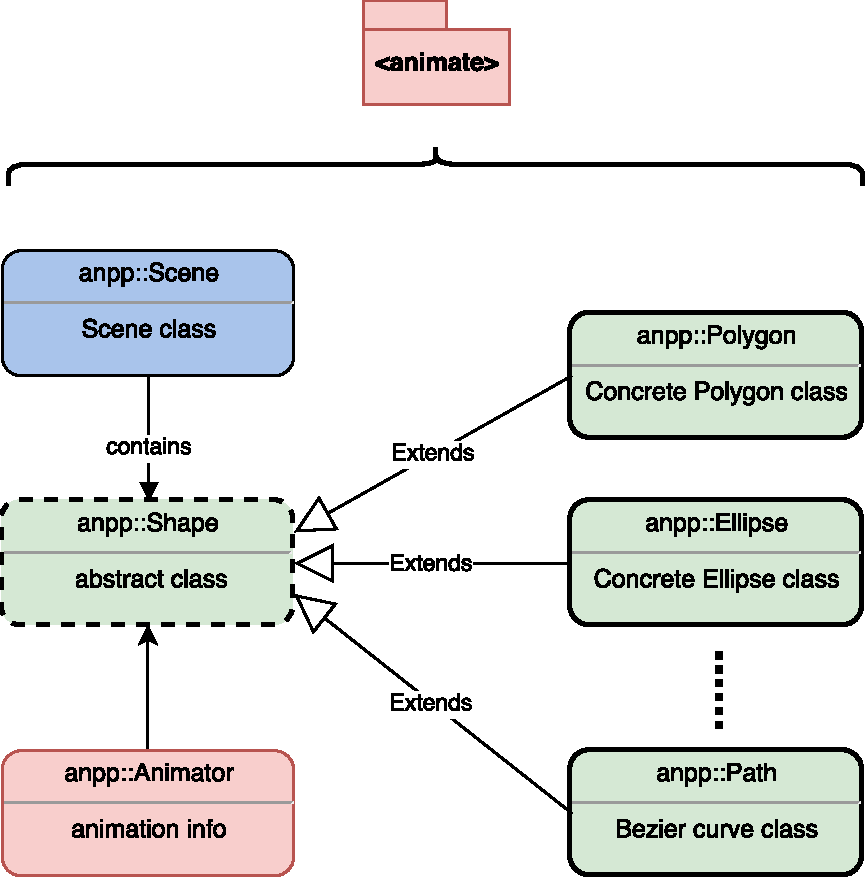
\includegraphics[width=6cm]{assets/animatepp-class-crop.pdf}
    \nocaptionrule \caption{\label{fig:class-diagram} Structure of \textsc{Animate++} class hierarchy.}
\end{figure}


We propose to build a C++ library, \textsc{Animate++}, with class structures that exploits inheritance, polymorphism, and many other modern C++ features and primitives for vector graphics animation (shown in Figure \ref{fig:class-diagram}). Specifically, we plan to build classes of graphical primitives with animation description objects attached, abstractions for other concepts such as scenes, and high-level functions to generate common animation elements.

\section{Team Member Resposibilities}

\begin{itemize}
    \item
    \textbf{Wode ``Nimo'' Ni}: system architecture, library interface design, graphics related implementation, implementation of demonstrations
    \item
    \textbf{Xuanyuan Zhang}: system implementation, test cases, implementation of demonstrations
\end{itemize}



%------------------------------------------------------------------------------
% bibliography

\FloatBarrier % prevent figures breaking the reference section

\bibliographystyle{unsrt}
\bibliography{bibliography}

\end{document}
